\section{Simulaciones}

{
\setbeamercolor{background canvas}{bg=beamer@blendedblue!30}
\begin{frame}
  % frame contents here
    \centering
  \Huge
  Simulaciones
\end{frame}
}

\begin{frame}
\frametitle{Modelo Propuesto}
\begin{itemize}
    \item Partículas puntuales en una celda de lado \(L\) con condiciones periódicas.
    \item Módulo de velocidad constante \(v = 0.03\).
    \item Direcciones \(\theta\) aleatorias a \(t=0\), \(\theta \in [0, 2\pi]\).
    \item Radio de interacción \(r = 1\).
    \item Generación de \(N\) partículas aleatoriamente a \(t = 0\).
\end{itemize}
\end{frame}



\begin{frame}
\frametitle{Comportamiento del Sistema}
\begin{itemize}
    \item Velocidad promedio normalizada \(v_a\) como observable.
    \[    v_a = \frac{1}{Nv} \left| \sum^{N}_{i=1} v_i \right|
\]
    \item Parámetros de interés: ruido \(\eta\) y densidad \(\rho = N / L^2\).
    \item \(v_a\) tiende a cero para desorden total y a 1 para partículas polarizadas.
\end{itemize}
\end{frame}

\begin{frame}
\frametitle{Simulaciones y Análisis}
\begin{itemize}
    \item Variación de \(v_a\) en función del ruido (\(\eta\)).
        \item Variación de \(v_a\) en función de la densidad (\(\rho\))
\end{itemize}
\end{frame}

\begin{frame}
\frametitle{Parámetros}
Comportamiento de \(v_a\) con ruido
    \begin{itemize}
    \item \(\eta \in [0, 5]\), \(N \in \{40, 100, 400\}\)
    \item Densidad constante \(\rho = 4\), ajuste \(L\) con \(N\).
    \end{itemize}
Comportamiento de \(v_a\) con densidad
    \begin{itemize}
    \item \(\rho \in [0, 10]\), \(L = 20\), \(\eta = 2.5\)
\end{itemize}

\end{frame}


\begin{frame}
\frametitle{Cálculo de \(v_a\) y Estado Estacionario}
\begin{itemize}
    \item Se calcula \(v_a\) cuando sistema esté estable.
    \item Se determina el tiempo estacionario con pruebas.
\end{itemize}
\end{frame}


\begin{frame}
\frametitle{Baja densidad}

\begin{columns}
    \begin{column}{0.7\textwidth}
      \begin{center}

\ifthenelse{\equal{\OUTPUT}{video}}
{\animategraphics[loop,controls,width=0.7\linewidth]{30}{animation/low_density/plot_}{0001}{1200}}
{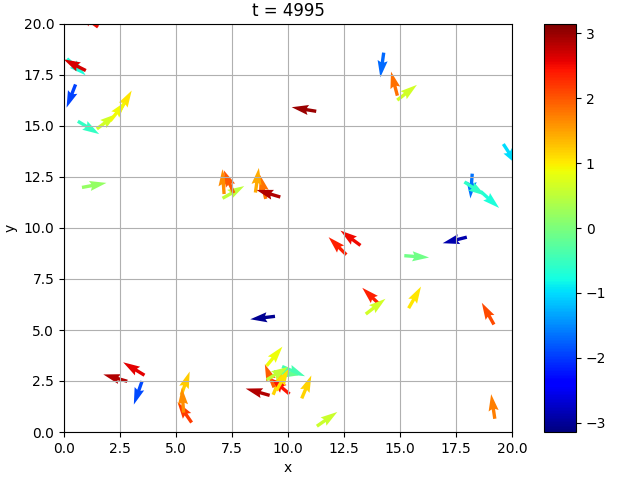
\includegraphics[width=0.7\linewidth]{animation/low_density/plot_1000.png}}

\end{center}
    \end{column}
    \begin{column}{0.3\textwidth}
\begin{center}
            \footnotesize
        \begin{itemize}
        \item \(L = 20\)
        \item \(\eta = 2.5\)
        \item \(N = 200\)
        \item \(\rho = 0.5\)
        \end{itemize}
\end{center}
    \end{column}
\end{columns}
\end{frame}

\begin{frame}
\frametitle{Alta densidad}

\begin{columns}
    \begin{column}{0.7\textwidth}
      \begin{center}
\ifthenelse{\equal{\OUTPUT}{video}}
{\animategraphics[loop,controls,width=0.7\linewidth]{30}{animation/high_density/plot_}{0001}{1200}}
{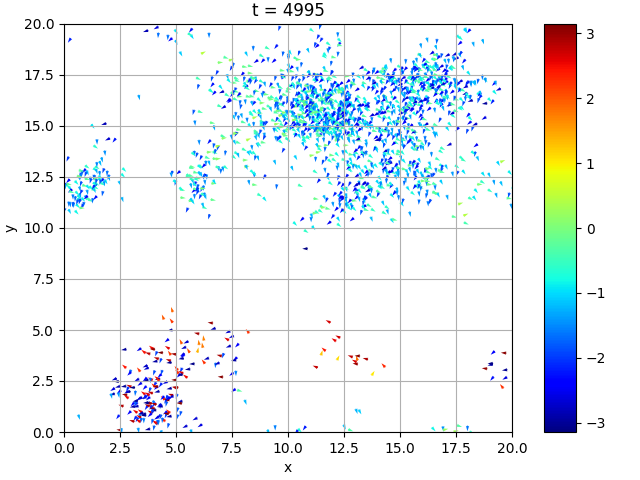
\includegraphics[width=0.7\linewidth]{animation/high_density/plot_1000.png}}
\end{center}
    \end{column}
    \begin{column}{0.3\textwidth}
\begin{center}
            \footnotesize
        \begin{itemize}
        \item \(L = 20\)
        \item \(\eta = 2.5\)
        \item \(N = 2000\)
        \item \(\rho = 5\)
        \end{itemize}
\end{center}
    \end{column}
\end{columns}
\end{frame}
\begin{frame}
\frametitle{Bajo ruido}

\begin{columns}
    \begin{column}{0.7\textwidth}
      \begin{center}
\ifthenelse{\equal{\OUTPUT}{video}}
{\animategraphics[loop,controls,width=0.7\linewidth]{30}{animation/low_noise/plot_}{0001}{1200}}
{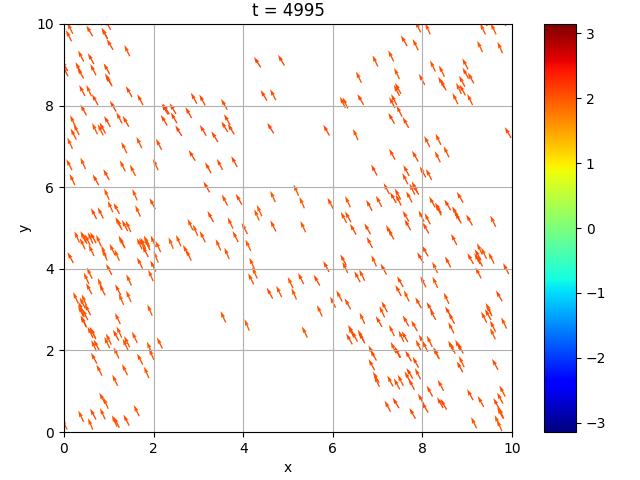
\includegraphics[width=0.7\linewidth]{animation/low_noise/plot_1000.png}}
\end{center}
    \end{column}
    \begin{column}{0.3\textwidth}
\begin{center}
            \footnotesize
        \begin{itemize}
        \item \(L = 10\)
        \item \(\eta = 0.1\)
        \item \(N = 400\)
        \item \(\rho = 4\)
        \end{itemize}
\end{center}
    \end{column}
\end{columns}
\end{frame}

\begin{frame}
\frametitle{Alto ruido}

\begin{columns}
    \begin{column}{0.7\textwidth}
      \begin{center}
\ifthenelse{\equal{\OUTPUT}{video}}
{\animategraphics[loop,controls,width=0.7\linewidth]{30}{animation/high_noise/plot_}{0001}{1200}}
{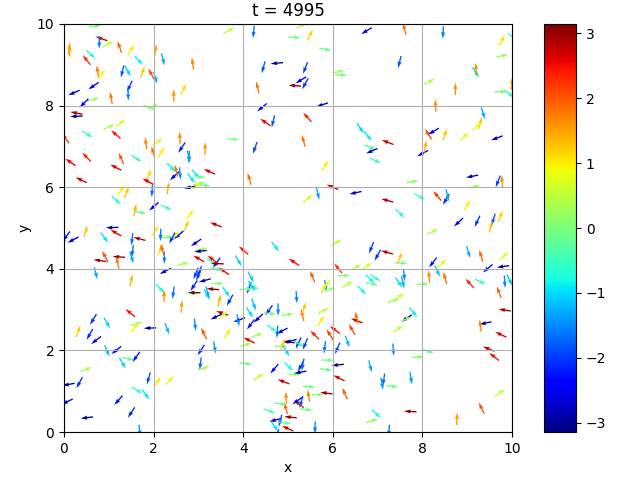
\includegraphics[width=0.7\linewidth]{animation/high_noise/plot_1000.png}}
\end{center}
    \end{column}
    \begin{column}{0.3\textwidth}
\begin{center}
            \footnotesize
        \begin{itemize}
        \item \(L = 10\)
        \item \(\eta = 5\)
        \item \(N = 400\)
        \item \(\rho = 4\)
        \end{itemize}
\end{center}
    \end{column}
\end{columns}
\end{frame}















